\section{System Perspective}
\subsection{Design and Architecture}
The system underwent multiple iterations as new technologies were incorporated into the tech stack. Therefore, in this section, we will present the overall system architecture.



\subsubsection{Servers and technology allocation}
Considering the system's integration of multiple technologies that required substantial CPU and memory resources on the Ubuntu server, specifically designed for enterprise-level systems, we opted to distribute some of the resource-intensive technologies among separate servers. Therefore, we determined which technologies would be deployed on the Docker Swarm, and which would be on separate servers. This decision was made to ensure consistent system availability and response time, even under the heavy load generated by simulated user traffic.

\begin{figure}[H]
  \centering
  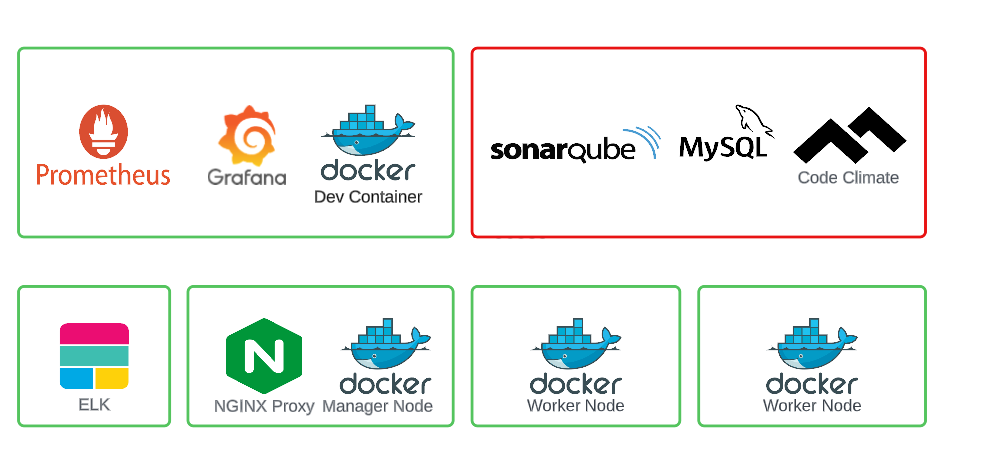
\includegraphics[width=1\textwidth]{images/system_perspective/Screenshot 2023-05-23 141829.png}
  \caption{Technologies allocation. Red indicating external service/managed. Green indicates one VM pr. square hosted Digital Ocean.}
  \label{fig:1}
\end{figure}

The ELK stack imposed significant demands on server specifications \parencite{ELK}. Hence, we needed to carefully manage our costs to remain within a budget of \$200 per user. Consequently, we set up a separate Digital Ocean account for this purpose, allowing us to allocate a server that met the specific requirements of the ELK stack. Despite its high minimum specifications, the log traffic did not have a substantial impact on the server's performance since the minimum requirements were sufficient to handle the workload efficiently.

Moreover, we made the decision to employ an additional server dedicated to Grafana and Prometheus. This choice aimed to efficiently and securely collect metrics from our Docker Swarm deployments. Additionally, this server served as a host for our developer container. Whenever a merge or push occurred in the development branch, the GitHub Action pipeline would automatically deploy a new container for testing purposes. This ensured that any changes were thoroughly evaluated before being rolled out in the production environment of our Docker Swarm.

Lastly, our Docker Swarm configuration consisted of one management node and two worker nodes. We selected the management node as the host for the NGINX reverse proxy, which served as a load balancer to evenly distribute incoming traffic across the servers, effectively allocating the workload.

To guarantee data integrity and alleviate the risk of resource shortage on our Ubuntu servers, we opted to procure a managed MySQL service from DigitalOcean. This choice provided built-in security measures, ensuring the safety of our data while preventing resource depletion.

We incorporated Code Churn and SonarQube into our system by utilizing their respective services and linking them to our GitHub repository. This integration allowed us to ensure the quality of our code and validate that it met the necessary requirements before being merged into the development branch for testing purposes or the main branch for production. Whenever a new build was triggered through the GitHub Action pipeline, these tools played a crucial role in analyzing the code and providing valuable insights.

\subsubsection{Design overview}

Figure \ref{fig:2} illustrates how incoming traffic is managed in our application. As mentioned previously, we utilize an NGINX reverse proxy that acts as a load balancer, distributing data in a round-robin fashion to our Docker manager and workers. This approach guarantees an even distribution of the load among the nodes, which then forward it to the respective tasks which distribute it to the replicated containers. These containers are responsible for processing the incoming data, executing the necessary business logic, and storing it in the managed MySQL database.
\begin{figure}[H]
  \centering
  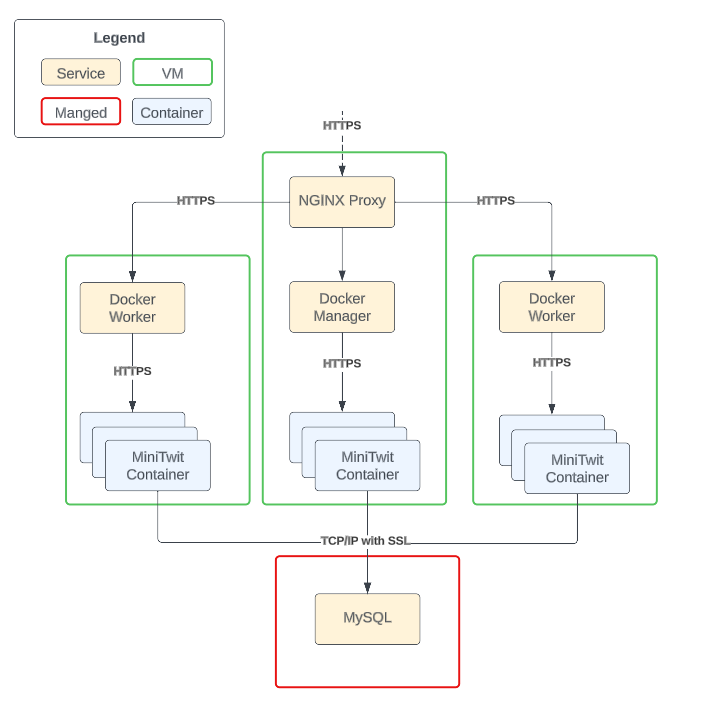
\includegraphics[width=0.60\textwidth]{images/system_perspective/OverView1.png}
  \caption{Component \& connector view - from incoming request to the system.}
  \label{fig:2}
\end{figure}
The logging and monitoring aspect, depicted in Figure \ref{fig:3}, showcases the communication within the system. It demonstrates how Prometheus interacts with the API exposed by the MiniTwit container to gather its metrics. This process occurs on a predetermined schedule, as Prometheus regularly checks for new metric data. Subsequently, Grafana retrieves the scraped data from Prometheus to create visualizations that provide us as developers with insights into the system's health and traffic.
\begin{figure}[H]
  \centering
  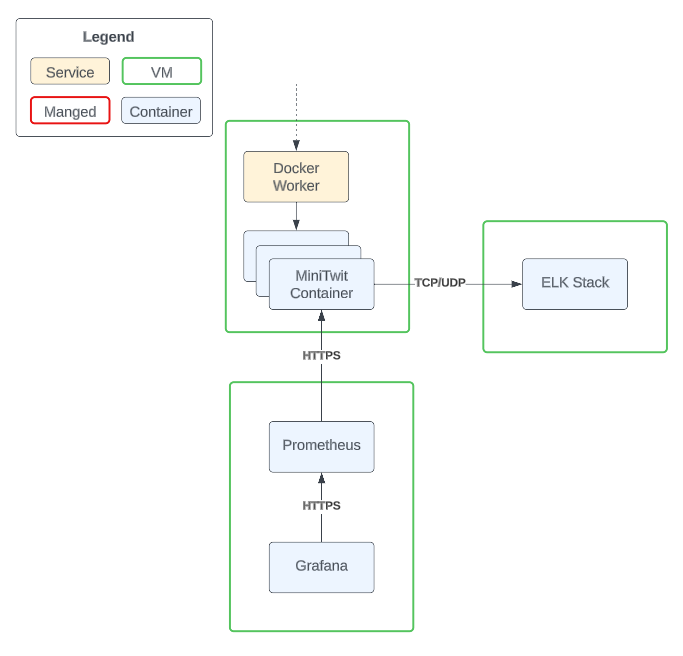
\includegraphics[width=0.65\textwidth]{images/system_perspective/OverViewZoom1.png}
  \caption{Component \& connector view - for scraping of metrics and logging.}
  \label{fig:3}
\end{figure}
Moreover, the containers in our system send relevant logs to our ELK stack, which proves valuable in identifying bugs and detecting warnings that may indicate an improper system state. This is visualized through Elasticsearch Search, allowing us to filter the log levels and facilitating bug detection.

\subsection{Dependencies}
In this section we will list the dependencies and technologies that we rely on for our application to work. It will be separated into application, infrastructure, and auxiliary software, and ordered by the point in time it was introduced. We will briefly discuss our choices after each subsection, for the most important dependencies. 
\subsubsection*{MiniTwit application}
\begin{itemize}
    \item \textbf{Week 02}
    \begin{itemize}
        \item Java 17
        \item Maven 3.8.4
        \item Spring Boot
        \item H2 Database
    \end{itemize}
    \item \textbf{Week 03}
    \begin{itemize}
        \item Maven 3.8.4
        \item Spring Boot
    \end{itemize}
\end{itemize}
\textbf{Java/Maven/Spring} - We landed on using Java with the Spring framework. Spring provides a web framework that made it easy to map the functionality from the original python MiniTwit, and it also provides easy integration with Docker for later containerization. It is also very commonly used in enterprise applications worldwide and specifically in Denmark, from our own job experience. Therefore using it while practicing DevOps will provide us with skills we will likely need in the future.

We did not consider benchmarking different languages/frameworks and picking the fastest, since it doesn't align with our motivations for taking the course. 

\subsubsection*{Infrastructure}
\begin{itemize}
    \item \textbf{Week 02}
    \begin{itemize}
        \item Git/GitHub
    \end{itemize}
    \item \textbf{Week 03}
    \begin{itemize}
        \item Ubuntu 22.04
        \item Docker
        \item Vagrant
    \end{itemize}
        \item \textbf{Week 04}
    \begin{itemize}
        \item GitHub Actions
        \item DockerHub
    \end{itemize}
        \item \textbf{Week 10}
    \begin{itemize}
        \item Docker Swarm
    \end{itemize}
\end{itemize}

\subsubsection*{Auxiliary software}
\begin{itemize}
    \item \textbf{Week 05}
        \begin{itemize}
            \item MySQL
        \end{itemize}
    \item \textbf{Week 06}
        \begin{itemize}
            \item Prometheus
            \item Grafana
        \end{itemize}
            \item \textbf{Week 07}
        \begin{itemize}
            \item SonarQube
            \item CodeClimate
        \end{itemize}
        \item \textbf{Week 08}
        \begin{itemize}
            \item ElasticSearch
            \item Filebeat
            \item Kibana
        \end{itemize}
        \item \textbf{Week 09}
        \begin{itemize}
            \item OWASP Zap
        \end{itemize}
\end{itemize}
\textbf{MySQL} - We opted to use a managed MySQL database as our DBMS. It fit nicely with the application, and the transition from H2 was smooth, since they are both SQL-based. The choice of a managed one versus self-hosted mainly came down to lowering the complexity of operations. We wanted a stable server or droplet for our database, and calculating the costs versus performance, we could get more value from a managed MySQL database compared to a separate droplet where we set it up ourselves. 

In general with infrastructure and auxiliary software, we prioritized getting the most out of our time. This often meant picking the same technologies as the ones used in the lectures/exercises, so we would not need to worry about compatibility issues. Often the time spent adjusting it to our setup was enough in and of itself. The reasons for our choices are outlined more thoroughly in the \href{https://github.com/Academic-Weapons/ITU2023-DevOps/tree/dev/worklogs}{worklogs folder} of our repository.

\subsection{State of the system}
Our application is available on \href{https://academicweapons.dk/}{academicweapons.dk}. 

From the course \href{146.190.207.33:3000}{simulator dashboard} we can gather that uor system has processed at least 12.484.621 requests during the course. During this time, we've had the following errors:

\begin{center}
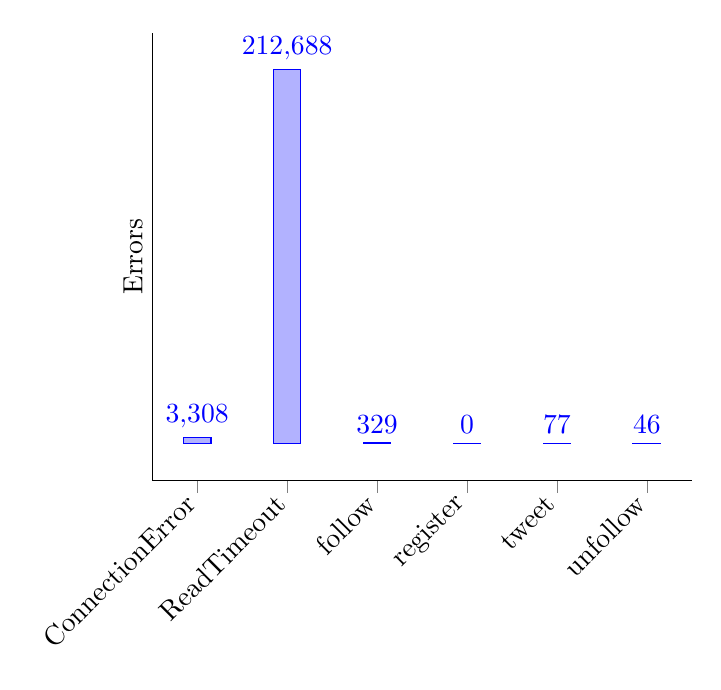
\begin{tikzpicture}
    \begin{axis}[
        ybar,
        ylabel={Errors},
        symbolic x coords={ConnectionError, ReadTimeout, follow, register, tweet, unfollow},
        xtick=data,
        nodes near coords,
        nodes near coords align={vertical},
        axis lines*=left, % this removes the right and top lines
        ytick=\empty, % this removes the y-axis labels
        x tick label style={rotate=45,anchor=east},
        nodes near coords style={/pgf/number format/fixed} % use fixed point notation
    ]
    \addplot coordinates {(ConnectionError, 3308) (ReadTimeout, 212688) (follow, 329) (register, 0) (tweet, 77) (unfollow, 46)};
    \end{axis}
\end{tikzpicture}
\end{center}
This data provides some interesting insights into the occurrence of the different types of errors. ReadTimeout (212688 occurrences) is by far the most common error. This might indicate some server performance issues or inefficient handling of requests in the system. It is more likely to be an issue with server performance or with the way requests are being handled. 

This is likely due to the fact that our budget constraints have caused us to choose smaller servers than perhaps was needed. Additionally, due to the operational expenses associated with maintaining DigitalOcean droplets, we have downscaled our system to the minimum requirements. If demand were to increase we can easily upscale the system to meet demand (as long as our budget allows us). Given its demanding minimum specifications, the ELK stack continues to operate on a robust, high-performance server. 


\subsection{License}
Our MiniTiwit relies on Spring Boot, licensed under Apache 2.0, allowing users to use, distribute, copy, and modify it \parencite{license}. The chosen MIT license is generally compatible with open-source licenses, and our open-source technologies align with its permissive nature. Thus, there are no conflicts with our direct dependencies' licenses.